\documentclass[spanish,letterpaper,oneside]{article}

% Datos del documento
\def\documenttitle {Volumen de prismas, pirámides y cilindros}
\def\documentsubtitle {Temas selectos de matemáticas I}
\def\documentsubject {Actividad 8 · Ficha y secuencia para exposición}
\def\documentauthor {Mtro. Martín Jonathan de la Cruz Muñoz}
\def\coursename {Temas selectos de matemáticas I}
\def\coursecode {PFM02}

% Identidad institucional
\def\universityname {Instituto de Investigación, Innovación y Estudios de Posgrado para la Educación del Estado de Nuevo León}
\def\universityfaculty {Maestría en Aprendizaje y Enseñanza de las Matemáticas}
\def\universitydepartment {Temas selectos de matemáticas I}
\def\universitydepartmentimage {img/iiiepe/marca-iiiepe.png}
\def\universitydepartmentimagecfg {height=1.75cm}
\def\universitylocation {Monterrey, Nuevo León}
\def\studentfullname {Mtro. Martín Jonathan de la Cruz Muñoz}
\def\studentid {00874}
\def\studentemail {martin.delacruz@campus.iiiepe.edu.mx}
\def\programperiod {1er tetramestre, marzo--julio de 2026}
\def\programmodality {Modalidad presencial}
\def\programshort {MAEM}

\def\authortable {
  \begin{tabular}{ll}
    \textbf{Alumno:} & \studentfullname \\
    Matrícula: & \studentid \\
    Correo institucional: & \studentemail \\
    Unidad: & \coursename \\
    Programa: & \programshort \\
    Periodo: & \programperiod \\
    & \\
    \multicolumn{2}{l}{Fecha de realización: 13 de octubre de 2026} \\
    \multicolumn{2}{l}{\universitylocation}
  \end{tabular}
}

\input{template}

\usepackage{helvet}
\renewcommand{\familydefault}{\sfdefault}
\usepackage{array}
\usepackage{longtable}
\usepackage{pdflscape}
\usepackage{tikz}
\usepackage[most]{tcolorbox}
\usetikzlibrary{arrows.meta,positioning,calc,fit,backgrounds}

\definecolor{iiiepeNavy}{HTML}{163B5C}
\definecolor{iiiepeBlue}{HTML}{1F6F9F}
\definecolor{iiiepeAqua}{HTML}{20B7A8}
\definecolor{iiiepeOrange}{HTML}{F28C28}
\definecolor{iiiepePaper}{HTML}{F6F8F7}
\definecolor{iiiepeInk}{HTML}{1E2A32}
\def\portraittitlecolor {iiiepeNavy}
\setcitestyle{authoryear,open={(},close={)}}

\newcommand{\insertcoverwatermark}{%
  \AddToShipoutPictureBG*{%
    \begin{tikzpicture}[remember picture,overlay]
      \node[opacity=.09,inner sep=0pt] at (current page.center)
      {\includegraphics[width=.58\paperwidth]{img/iiiepe/logo-puntos.png}};
    \end{tikzpicture}%
  }%
}

\newtcolorbox{reportelecturabox}[1][]{%
  enhanced,breakable,
  colback=iiiepePaper,colframe=iiiepeNavy,
  boxrule=1pt,leftrule=4pt,arc=2pt,
  left=8pt,right=8pt,top=6pt,bottom=6pt,
  before skip=6pt,after skip=10pt,
  fonttitle=\bfseries\color{white},coltitle=white,
  colbacktitle=iiiepeNavy,
  attach boxed title to top left={xshift=8pt,yshift=-2pt},
  boxed title style={colback=iiiepeNavy,colframe=iiiepeNavy,arc=1pt},
  title={Reporte de lectura},#1}

\newtcolorbox{fichalecturabox}[1][]{%
  enhanced,breakable,
  colback=iiiepeAqua!7,colframe=iiiepeAqua!70!iiiepeNavy,
  boxrule=.6pt,arc=1pt,
  left=7pt,right=7pt,top=4pt,bottom=4pt,
  fontupper=\small,before upper={\setstretch{1.0}},
  fonttitle=\bfseries\color{iiiepeNavy},coltitle=iiiepeNavy,
  colbacktitle=iiiepeAqua!7,
  title={Ficha de la lectura},#1}



\usepackage{tabularx,colortbl,pgfplots,enumitem,needspace}\pgfplotsset{compat=1.18}\definecolor{iiiepePale}{HTML}{EEF5F8}
\setlength{\parskip}{5pt}\setlength{\parindent}{0pt}
\begin{document}\insertcoverwatermark\templatePortrait\templatePagecfg\templateFinalcfg\fancyfoot{}\fancyfoot[L]{\scriptsize IIIEPE · MAEM}\fancyfoot[C]{\scriptsize\thepage}\fancyfoot[R]{\scriptsize Actividad 8}\setstretch{1.3}\raggedbottom
\section{Reto y propósito}
Se propone comparar recipientes con la misma base y altura para comprender volumen de prismas, cilindros y pirámides. El PDA exige usar diferentes estrategias de cálculo, por lo que el producto combina unidades cúbicas, fórmulas, despejes y relaciones de variación. Un contexto de diseño de depósitos conecta el tema con mantenimiento e ingeniería sin convertir el aprendizaje en una simple aplicación de recetas.

\begin{center}
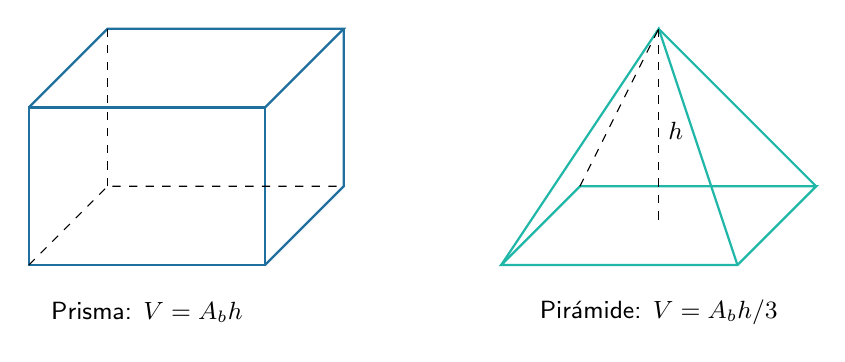
\begin{tikzpicture}[font=\small,x=1cm,y=1cm]
\draw[thick,iiiepeBlue] (0,0)--(3,0)--(3,2)--(0,2)--cycle;\draw[thick,iiiepeBlue] (0,2)--(1,3)--(4,3)--(3,2);\draw[thick,iiiepeBlue] (3,0)--(4,1)--(4,3);\draw[dashed] (0,0)--(1,1)--(4,1);\draw[dashed] (1,1)--(1,3);
\node at (1.5,-.6){Prisma: $V=A_bh$};\draw[thick,iiiepeAqua] (6,0)--(9,0)--(10,1)--(7,1)--cycle;\draw[thick,iiiepeAqua] (6,0)--(8,3)--(9,0);\draw[thick,iiiepeAqua] (10,1)--(8,3);\draw[dashed] (7,1)--(8,3);\draw[dashed] (8,3)--(8,.5);\node[right] at (8,1.7){$h$};\node at (8,-.6){Pirámide: $V=A_bh/3$};\end{tikzpicture}
\end{center}
\section{Fases 1 y 2 · Estimación e indagación}
La pregunta inicial es si una pirámide y un prisma con igual base y altura tienen igual capacidad. Primero se estima y después se contrasta mediante un modelo de llenado. El experimento propuesto utilizaría arena o arroz y recipientes con geometría controlada. No se reportan mediciones físicas realizadas.
Las fórmulas ideales son $V_{prisma}=A_bh$, $V_{cilindro}=\pi r^2h$ y $V_{pirámide}=A_bh/3$. El factor $1/3$ corresponde a pirámides; no debe aplicarse a todos los cuerpos que terminan en punta sin identificar su geometría.
\section{Fase 3 · Problemas resueltos}


{\small\setstretch{1.1}\renewcommand{\arraystretch}{1.25}
\begin{longtable}{|>{\raggedright\arraybackslash}p{\dimexpr0.5\linewidth-2\tabcolsep-2\arrayrulewidth\relax}|>{\raggedright\arraybackslash}p{\dimexpr0.5\linewidth-2\tabcolsep-2\arrayrulewidth\relax}|}\hline
\rowcolor{iiiepePale} \textbf{Cuerpo o pregunta} & \textbf{Cálculo y respuesta} \\\hline
\endfirsthead
\hline
\rowcolor{iiiepePale} \textbf{Cuerpo o pregunta} & \textbf{Cálculo y respuesta} \\\hline
\endhead
Cubo de arista 4 cm & $V=4^3=64$ cm$^3$. \\\hline
Prisma de $8\times5\times3$ cm & $V=(8\cdot5)(3)=120$ cm$^3$. \\\hline
Pirámide con la misma base y altura & $V=(1/3)(40)(3)=40$ cm$^3$. \\\hline
Cilindro con $r=3$ cm y $h=10$ cm & $V=\pi(3)^2(10)=90\pi\approx282.74$ cm$^3$. \\\hline
Altura de prisma con $V=240$ y $A_b=40$ & $h=V/A_b=240/40=6$ cm. \\\hline
Altura de pirámide con $V=96$ y $A_b=36$ & $h=3V/A_b=288/36=8$ cm. \\\hline
Radio de cilindro con $V=500\pi$ cm$^3$, $h=20$ cm & $r=\sqrt{V/(\pi h)}=\sqrt{25}=5$ cm. \\\hline
\end{longtable}}


\section{Fase 4 · Variación y comunicación}
Con área de base fija, duplicar la altura duplica el volumen de prismas y pirámides: la relación con $h$ es directa. Con altura fija, duplicar el radio de un cilindro cuadruplica su volumen porque el radio aparece al cuadrado. Duplicar todas las dimensiones multiplica el volumen por $2^3=8$ y el área por $2^2=4$; un diseño a escala no conserva estas magnitudes con el mismo factor.


{\small\setstretch{1.1}\renewcommand{\arraystretch}{1.25}
\begin{longtable}{|>{\raggedright\arraybackslash}p{\dimexpr0.5\linewidth-2\tabcolsep-2\arrayrulewidth\relax}|>{\raggedright\arraybackslash}p{\dimexpr0.5\linewidth-2\tabcolsep-2\arrayrulewidth\relax}|}\hline
\rowcolor{iiiepePale} \textbf{Radio del cilindro (cm)} & \textbf{Volumen con $h=10$ cm} \\\hline
\endfirsthead
\hline
\rowcolor{iiiepePale} \textbf{Radio del cilindro (cm)} & \textbf{Volumen con $h=10$ cm} \\\hline
\endhead
1 & $10\pi$ cm$^3$ \\\hline
2 & $40\pi$ cm$^3$ \\\hline
3 & $90\pi$ cm$^3$ \\\hline
4 & $160\pi$ cm$^3$ \\\hline
\end{longtable}}


Para un depósito rectangular de $0.8\times0.5\times0.3$ m, $V=0.12$ m$^3=120$ L. Si se requiere 10\% de volumen libre, la capacidad operativa propuesta es 108 L. El espacio libre es una condición de diseño del ejemplo, no un requisito de la plataforma ni una norma industrial.
\section{Volumen, semejanza y despeje}
El factor de escala se deduce de la estructura de la fórmula. Un prisma con dimensiones $a,b,h$ tiene $V=abh$. Si todas se multiplican por $s$, el nuevo volumen es $(sa)(sb)(sh)=s^3V$. Para $s=2$, el resultado es ocho veces el volumen original. En cambio, si solo cambia la altura, el factor es $s$, porque las dimensiones de la base permanecen constantes.
En una pirámide con $V=96$ cm$^3$ y $A_b=36$ cm$^2$, partir de $V=A_bh/3$ conduce a $3V=A_bh$ y a $h=3V/A_b=8$ cm. El cociente de cm$^3$ entre cm$^2$ tiene unidad cm; esta comprobación dimensional ayuda a detectar una fórmula invertida.
El factor $1/3$ requiere una exploración geométrica o de llenado con bases y alturas comparables. No basta mostrar dos recipientes que se parezcan. La actividad debe permitir anticipar, contrastar y explicar; si no se dispone de cuerpos adecuados, se utilizará un modelo geométrico y se declarará el límite de la demostración experimental.
\section{Secuencia de aplicación y evaluación}
Calcular volúmenes y explicar variación de dimensiones. La duración propuesta es de 80 minutos, ajustable al diagnóstico y a los recursos. Esta planeación sigue la progresión de los recursos institucionales (IIIEPE, 2026); los tiempos y apoyos son decisiones de codiseño, no datos de una aplicación ya realizada.

{\small\setstretch{1.1}\renewcommand{\arraystretch}{1.25}
\begin{longtable}{|>{\raggedright\arraybackslash}p{\dimexpr0.23\linewidth-2\tabcolsep-2\arrayrulewidth\relax}|>{\raggedright\arraybackslash}p{\dimexpr0.49\linewidth-2\tabcolsep-2\arrayrulewidth\relax}|>{\raggedright\arraybackslash}p{\dimexpr0.28\linewidth-2\tabcolsep-2\arrayrulewidth\relax}|}\hline
\rowcolor{iiiepePale} \textbf{Fase y tiempo} & \textbf{Actividad y mediación} & \textbf{Evidencia} \\\hline
\endfirsthead
\hline
\rowcolor{iiiepePale} \textbf{Fase y tiempo} & \textbf{Actividad y mediación} & \textbf{Evidencia} \\\hline
\endhead
1. Reto y saberes (10 min) & Estimar capacidades de cuerpos de igual base y altura. & Predicción individual y pregunta. \\\hline
2. Plan de indagación (15 min) & Relacionar unidades cúbicas con las fórmulas y sus condiciones. & Plan explicado y criterios. \\\hline
3. Construcción y análisis (25 min) & Resolver un volumen y despejar una dimensión desconocida. & Registro o procedimiento trazable. \\\hline
4. Comunicación y aplicación (18 min) & Predecir el efecto de duplicar una o todas las dimensiones. & Argumento con comprobación. \\\hline
5. Metacognición (12 min) & Corregir un error de escala y explicar la diferencia entre área y volumen. & Versión revisada y justificación. \\\hline
\end{longtable}}
\subsection{Criterios observables y retroalimentación}

{\small\setstretch{1.1}\renewcommand{\arraystretch}{1.25}
\begin{longtable}{|>{\raggedright\arraybackslash}p{\dimexpr0.22\linewidth-2\tabcolsep-2\arrayrulewidth\relax}|>{\raggedright\arraybackslash}p{\dimexpr0.4\linewidth-2\tabcolsep-2\arrayrulewidth\relax}|>{\raggedright\arraybackslash}p{\dimexpr0.38\linewidth-2\tabcolsep-2\arrayrulewidth\relax}|}\hline
\rowcolor{iiiepePale} \textbf{Criterio} & \textbf{Evidencia de logro} & \textbf{Acción si necesita apoyo} \\\hline
\endfirsthead
\hline
\rowcolor{iiiepePale} \textbf{Criterio} & \textbf{Evidencia de logro} & \textbf{Acción si necesita apoyo} \\\hline
\endhead
Identificación del cuerpo & Explica identificación del cuerpo con un caso de la actividad. & Pedir una representación concreta y contrastar dos casos. \\\hline
Fórmula y despeje & Conserva fórmula y despeje en el desarrollo y justifica sus pasos. & Modelar un paso, retirar gradualmente la ayuda y solicitar otro caso. \\\hline
Unidades & Utiliza unidades para contrastar una respuesta o representación. & Comparar la evidencia inicial y la corregida con una pregunta específica. \\\hline
Escala y variación & Relaciona escala y variación con la conclusión y un límite del problema. & Solicitar una comprobación independiente y un caso de transferencia. \\\hline
\end{longtable}}
El instrumento es una propuesta docente. Cada criterio se registra como logrado con autonomía, logrado con apoyo o aún no demostrado; no se asigna una calificación observada sin aplicar la actividad. En la coevaluación, un compañero verifica un criterio y formula una pregunta; en la autoevaluación, el estudiante explica una corrección; el docente contrasta ambas evidencias y decide el siguiente apoyo.\subsection{Participación y apoyos}
La inclusión se concreta en alternativas de representación y de acceso; el pensamiento crítico, en justificar y contrastar. Los roles de cálculo, registro y explicación se rotan para que todos produzcan una evidencia individual. Quien necesita apoyo dispone de un ejemplo parcial y preguntas graduadas; quien ya domina el procedimiento analiza un contraejemplo o cambia una condición. Estas acciones deben observarse durante la aplicación para valorar su funcionamiento.

\section{Fase 5 · Metacognición y reflexión pedagógica}
El cierre pediría explicar el factor $1/3$, resolver una medida desconocida y discutir por qué duplicar el radio no duplica el volumen. Evaluaría que cada despeje conserve unidades y que una fórmula se relacione con una representación del cuerpo. Los estudiantes podrían verificar entre pares un cálculo y corregirlo antes de una tarea de transferencia.
Diseñaría estaciones con material manipulable, dibujo y cálculo para que todos participen. La experiencia técnica aporta contextos; el enfoque humanista evita que la familiaridad previa con herramientas determine el éxito. La mejora se observaría en las explicaciones revisadas y no se inferiría únicamente de un envase atractivo.

\needspace{5\baselineskip}\section*{Referencias}
{\setstretch{1.15}\setlength{\parskip}{6pt}
\par\hangindent=1.27cm\hangafter=1  IIIEPE. (2026). \textit{Sesión 8: Medición y cálculo en diferentes contextos}. EVA posgrado.
\par\hangindent=1.27cm\hangafter=1  Secretaría de Educación Pública. (2024). \textit{Programa de estudio para la educación secundaria: Programa sintético de la Fase 6}. SEP.
}

\end{document}
